%%%%%%%%%%%%%%%%%%%%%%%%%%%%%%%%%%%%%%%%%
% Programming/Coding Assignment
% LaTeX Template
%
% This template has been downloaded from:
% http://www.latextemplates.com
%
% Original author:
% Ted Pavlic (http://www.tedpavlic.com)
%
% Note:
% The \lipsum[#] commands throughout this template generate dummy text
% to fill the template out. These commands should all be removed when 
% writing assignment content.
%
% This template uses a Perl script as an example snippet of code, most other
% languages are also usable. Configure them in the "CODE INCLUSION 
% CONFIGURATION" section.
%
%%%%%%%%%%%%%%%%%%%%%%%%%%%%%%%%%%%%%%%%%

%----------------------------------------------------------------------------------------
%	PACKAGES AND OTHER DOCUMENT CONFIGURATIONS
%----------------------------------------------------------------------------------------

\documentclass{article}

\usepackage[T1]{fontenc}
\usepackage[polish]{babel}
\usepackage[utf8]{inputenc}
\usepackage{lmodern}
\selectlanguage{polish}

\usepackage{float}

\usepackage{fancyhdr} % Required for custom headers
\usepackage{lastpage} % Required to determine the last page for the footer
\usepackage{extramarks} % Required for headers and footers
\usepackage[usenames,dvipsnames]{color} % Required for custom colors
\usepackage{graphicx} % Required to insert images
\usepackage{listings} % Required for insertion of code
\usepackage{courier} % Required for the courier font
\usepackage{lipsum} % Used for inserting dummy 'Lorem ipsum' text into the template

% Margins
\topmargin=-0.45in
\evensidemargin=0in
\oddsidemargin=0in
\textwidth=6.5in
\textheight=9.0in
\headsep=0.25in

\linespread{1.1} % Line spacing

% Set up the header and footer
\pagestyle{fancy}
\lhead{\hmwkAuthorName} % Top left header
\rhead{\firstxmark} % Top right header
\lfoot{\lastxmark} % Bottom left footer
\cfoot{} % Bottom center footer
\rfoot{Strona\ \thepage\ z \protect\pageref{LastPage}} % Bottom right footer
\renewcommand\headrulewidth{0.4pt} % Size of the header rule
\renewcommand\footrulewidth{0.4pt} % Size of the footer rule

\setlength\parindent{0pt} % Removes all indentation from paragraphs

%----------------------------------------------------------------------------------------
%	CODE INCLUSION CONFIGURATION
%----------------------------------------------------------------------------------------

\definecolor{MyDarkGreen}{rgb}{0.0,0.4,0.0} % This is the color used for comments
\lstloadlanguages{Perl} % Load Perl syntax for listings, for a list of other languages supported see: ftp://ftp.tex.ac.uk/tex-archive/macros/latex/contrib/listings/listings.pdf
\lstset{language=R,
        frame=single, % Single frame around code
        basicstyle=\small\ttfamily, % Use small true type font
        keywordstyle=[1]\color{Blue}\bf, % Perl functions bold and blue
        keywordstyle=[2]\color{Purple}, % Perl function arguments purple
        keywordstyle=[3]\color{Blue}\underbar, % Custom functions underlined and blue
        identifierstyle=, % Nothing special about identifiers                                         
        commentstyle=\usefont{T1}{pcr}{m}{sl}\color{MyDarkGreen}\small, % Comments small dark green courier font
        stringstyle=\color{Purple}, % Strings are purple
        showstringspaces=false, % Don't put marks in string spaces
        tabsize=5, % 5 spaces per tab
        %
        % Put standard Perl functions not included in the default language here
        morekeywords={rand},
        %
        % Put Perl function parameters here
        morekeywords=[2]{on, off, interp},
        %
        % Put user defined functions here
        morekeywords=[3]{test},
       	%
        morecomment=[l][\color{Blue}]{...}, % Line continuation (...) like blue comment
        numbers=left, % Line numbers on left
        firstnumber=1, % Line numbers start with line 1
        numberstyle=\tiny\color{Blue}, % Line numbers are blue and small
        stepnumber=5 % Line numbers go in steps of 5
}

% Creates a new command to include a perl script, the first parameter is the filename of the script (without .pl), the second parameter is the caption
\newcommand{\rscript}[2]{
\begin{itemize}
\item[]\lstinputlisting[caption=#2,label=#1]{kod/#1.r}
\end{itemize}
}

%----------------------------------------------------------------------------------------
%	DOCUMENT STRUCTURE COMMANDS
%	Skip this unless you know what you're doing
%----------------------------------------------------------------------------------------

% Header and footer for when a page split occurs within a problem environment
\newcommand{\enterProblemHeader}[1]{
\nobreak\extramarks{#1}{#1 continued on next page\ldots}\nobreak
\nobreak\extramarks{#1 (continued)}{#1 continued on next page\ldots}\nobreak
}

% Header and footer for when a page split occurs between problem environments
\newcommand{\exitProblemHeader}[1]{
\nobreak\extramarks{#1 (continued)}{#1 continued on next page\ldots}\nobreak
\nobreak\extramarks{#1}{}\nobreak
}

\setcounter{secnumdepth}{0} % Removes default section numbers
\newcounter{homeworkProblemCounter} % Creates a counter to keep track of the number of problems

\newcommand{\homeworkProblemName}{}
\newenvironment{homeworkProblem}[1][Problem \arabic{homeworkProblemCounter}]{ % Makes a new environment called homeworkProblem which takes 1 argument (custom name) but the default is "Problem #"
\stepcounter{homeworkProblemCounter} % Increase counter for number of problems
\renewcommand{\homeworkProblemName}{#1} % Assign \homeworkProblemName the name of the problem
\section{\homeworkProblemName} % Make a section in the document with the custom problem count
\enterProblemHeader{\homeworkProblemName} % Header and footer within the environment
}{
\exitProblemHeader{\homeworkProblemName} % Header and footer after the environment
}

\newcommand{\problemAnswer}[1]{ % Defines the problem answer command with the content as the only argument
\noindent\framebox[\columnwidth][c]{\begin{minipage}{0.98\columnwidth}#1\end{minipage}} % Makes the box around the problem answer and puts the content inside
}

\newcommand{\homeworkSectionName}{}
\newenvironment{homeworkSection}[1]{ % New environment for sections within homework problems, takes 1 argument - the name of the section
\renewcommand{\homeworkSectionName}{#1} % Assign \homeworkSectionName to the name of the section from the environment argument
\subsection{\homeworkSectionName} % Make a subsection with the custom name of the subsection
\enterProblemHeader{\homeworkProblemName\ [\homeworkSectionName]} % Header and footer within the environment
}{
\enterProblemHeader{\homeworkProblemName} % Header and footer after the environment
}

%----------------------------------------------------------------------------------------
%	NAME AND CLASS SECTION
%----------------------------------------------------------------------------------------

\newcommand{\hmwkTitle}{} % Assignment title
\newcommand{\hmwkDueDate}{Rozpoznawanie typu Pokemona po jego cechach.} % Due date
\newcommand{\hmwkClass}{Eksploracja Danych} % Course/class
\newcommand{\hmwkClassTime}{} % Class/lecture time
\newcommand{\hmwkClassInstructor}{} % Teacher/lecturer
\newcommand{\hmwkAuthorName}{Adam Kasperowicz - 279046 , Mateusz Sieczko - numerek} % Your name

%----------------------------------------------------------------------------------------
%	TITLE PAGE
%----------------------------------------------------------------------------------------

\title{
\vspace{2in}
\textmd{\textbf{\hmwkClass\ \hmwkTitle}}\\
\normalsize\vspace{0.1in}\small{Temat:\ \hmwkDueDate}\\
\vspace{0.1in}\large{\textit{\hmwkClassInstructor\ \hmwkClassTime}}
\vspace{3in}
}

\author{\textbf{\hmwkAuthorName}}
\date{} % Insert date here if you want it to appear below your name

%----------------------------------------------------------------------------------------

\begin{document}

\maketitle

%----------------------------------------------------------------------------------------
%	TABLE OF CONTENTS
%----------------------------------------------------------------------------------------

%\setcounter{tocdepth}{1} % Uncomment this line if you don't want subsections listed in the ToC

\newpage
\tableofcontents
\newpage

%----------------------------------------------------------------------------------------
%	Projekt
%----------------------------------------------------------------------------------------

% To have just one problem per page, simply put a \clearpage after each problem

\section{Problem}

Celem projektu jest klasyfikacja typu pokemonów na podstawie ich atrybutów. Oznacza to, że powinniśmy mieć możliwość określenia typu pokemona wyłącznie po jego atrybutach. 

Następujące prace zostaną wykonane:
\begin{enumerate}
	\item Analiza i zrozumienie posiadanych danych
	\item Obróbka danych w celu zmaksymalizowanie użyteczności posiadanych danych
	\item Wybranie najlepszego klasyfikatora
\end{enumerate}

\section{Analiza danych}

\subsection{Struktura danych}
\rscript{str}{Struktura danych}

Plik ``Pokemon.csv'' zawiera 800 obiektów, z których każdy opisany jest przez 13 atrybutów. Atrybuty są zarówno typu numerycznego, binarnego jak i łańcuchowego. 

Niektóre z atrybutów wymagają głębszego wyjaśnienia.
\begin{itemize}
	\item \textbf{X} - Atrybut ID zliczający ile w zbiorze istnieje pokemonów o niepowtarzalnym atrybucie name.
	\item \textbf{Name, Type.1, Type.2} - Atrybuty łańcuchowe które razem specyfikują jednoznacznie każdego pokemona. Atrybut \textbf{Type.2} pojawia się tylko wyjątkowo dla pokemonów posiadających więcej niż jeden typ. Dlatego, często gdy nie ma potrzeby dokładniejszej specyfikacji ten atrybut jest pusty.
	\item \textbf{Total, HP, Attack, Defense, Sp. Atk,Sp. Def, Speed, Generation} - Atrybuty będące liczbami całkowitymi opisują statystki danego pokemona. Każdy z pokemonów ma ten zestaw zmiennych w pełni wypełniony.
	\item \textbf{Legendary} - Atrybut binarny przyjmujący wartość True dla pokemonów legendarnych. Widzimy, że ten atrybut chociaż w większości przypadków będzie miał wartość równą False niesie bardzo ważną informację.
\end{itemize} 

\clearpage

Po przebadaniu struktury danych możemy ustalić parę ważnych faktów.
\begin{itemize}
	\item W zbiorze danych znajduje się 18 klas. Jest to ilość niepowtarzalnych elementów atrybutu \textbf{Type.1}
	\item Atrybut \textbf{X} musi zostać usunięty, gdyż był prawdopodobnie przydzielany arbitralnie i nie przekazuje żadnej informacji.
	\item Atrybut \textbf{Legendary} jest typu łańcuchowego i będzie musiał zostać zmieniony na typ liczb całkowitych o zakresie [0,1].
	\item Atrybut \textbf{Name} jest specyficzny pod tym względem, że prawie jednoznacznie wyznacza klasę obiektu. Atrybut ten sprawia, że problem klasyfikacji praktycznie znika, gdyż już po tylko tej zmiennej możemy określić typ pokemona. Na potrzeby projektu będziemy musieli wykluczyć ten atrybut z procesu klasyfikacji.
	\item Do klasyfikacji będziemy używać wszystkich atrybutów oprócz \textbf{X} i \textbf{Name}  
\end{itemize}

\subsection{Analiza graficzna}

Do przedstawienia danych w sposób graficzny posłużymy się dwuwymiarowymi wykresami oraz wykresami pudełkowymi. Z racji na swoją naturę graficznie przedstawione zostaną tylko atrybuty \textbf{Total, HP, Attack, Defense, Sp. Atk,Sp. Def, Speed, Generation}. Jako zmienna decyzyjna, jednocześnie koloryzująca punkty na wykresie, wykorzystana jest zmienna \textbf{Type.1}
\begin{figure}[H]
	\caption{Wykresy dwuwymiarowe}
	\begin{center}
	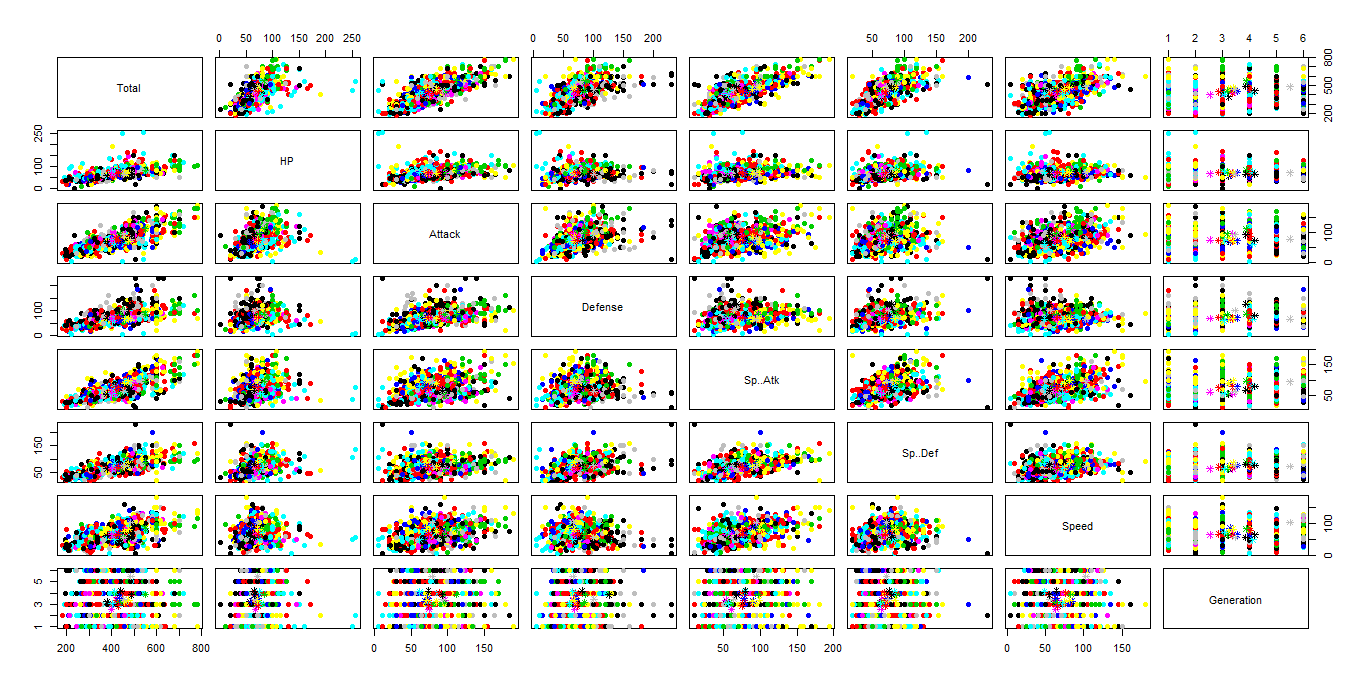
\includegraphics[width=1\columnwidth]{obrazki/graph} % Example image
	\end{center}
\end{figure}
\begin{figure}[H]
	\caption{Wykresy pudełkowe}
	\begin{center}
	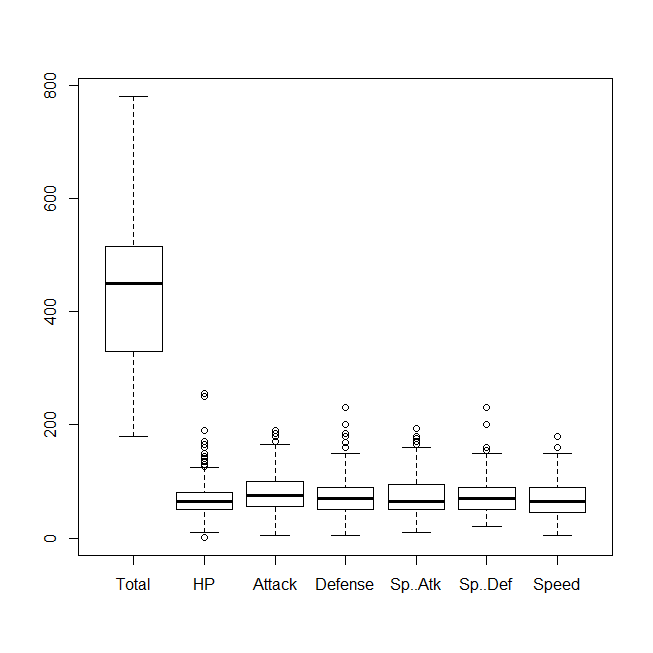
\includegraphics[width=0.75\columnwidth]{obrazki/boxplot} % Example image
	\end{center}
\end{figure}

Z wykresów wyciągamy następujące wnioski.
\begin{enumerate}
	\item Dane są generalnie równo rozłożone z paroma wartościami oddalonymi. Te nietypowe osobniki są to prawdopodobnie wyspecjalizowane lub ponadprzeciętnie silne pokemony. 
	\item Widzimy, że niektóre atrybuty są ze sobą silnie dodatnio skorelowane np. \textbf{Sp..Def i  Total} a niektóre praktycznie w ogóle np. \textbf{HP i Attack}.
	\item Wszystkie atrybuty przyjmują wartości z tego samego przedziału, wyjątkiem jest \textbf{Total} który będąc sumą pozostałych atrybutów musi się znacząco wywyższać. Z powodu tego jednego atrybutu będziemy musieli znormalizować dane. Inaczej wartości atrybutu \textbf{Total} dominowały by nad innymi atrybutami.
	\item Nie widać żadnych szczególnych zgrupowań które pozwoliły by podzielić pokemony na jakieś większe podgrupy.
\end{enumerate}

\clearpage

\subsection{Analiza ilościowa}

Kolejnym etapem jest próba skwantyfikowania obserwacji z poprzednich etapów.

\rscript{summary}{Podsumowanie danych}
\rscript{cor}{Korelacje}

\clearpage
Widzimy potwierdzenie naszych obserwacji w postaci numerycznej
\begin{itemize}
	\item Atrybuty liczbowe przyjmują wartości które widzieliśmy na wykresie pudełkowym
	\item Istnieje jedna kolumna z pustymi polami i jest to \textbf{Type.2}. Zauważamy jednak, że jest to dla nas nadal informacja i dla tego nie musimy tych pustych pól wypełniać.
	\item W zbiorze danych istnieje 6 generacji pokemonów. Jest to ważna informacja która w sama sobie pozwala nam na pogrupowanie wszystkich pokemonów na 6 grup.
	\item Pokemonów legendarnych jest znacznie mniej niż pokemonów zwyczajnych
	\item Nasze obserwacje na temat korelacji atrybutów zostają potwierdzone przez liczby. Warta głębszej uwagi jest zmienna \textbf{Total} będąca sumą pozostałych atrybutów liczbowych niespecjalnych. Pomimo silnej korelacji z jej składowymi atrybut daje nam nową informację i pozwala na lepszą klasyfikację.
\end{itemize}

\section{Przygotowanie danych}

\subsection{Obróbka danych}
Po przebadaniu danych możemy przejść do procesu obróbki. 

\rscript{obrob}{Obrabianie danych}

Nie istnieją braki w danych. 

\clearpage
\subsection{Grupowanie danych}

Jesteśmy gotowi sprawdzić z jaką łatwością dane się grupują.
Zaczynamy od próby zgrupowania danych względem atrybutu decyzyjnego, czyli \textbf{Type.1}

\begin{figure}[H]
	\caption{Grupowanie metodą kśrednich}
	\begin{center}
	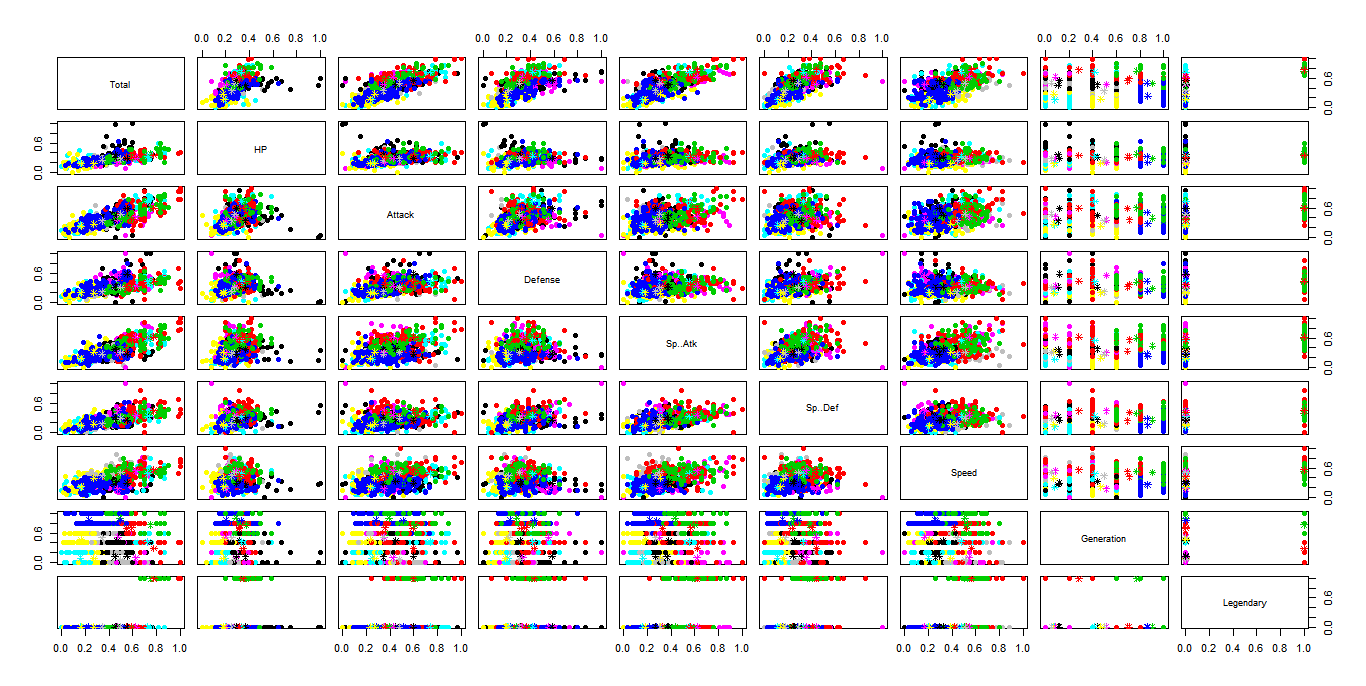
\includegraphics[width=1\columnwidth]{obrazki/ksrednie} % Example image
	\end{center}
\end{figure}
\begin{figure}[H]
	\caption{Grupowanie metodą hierarchiczną średniego połączenia}
	\begin{center}
	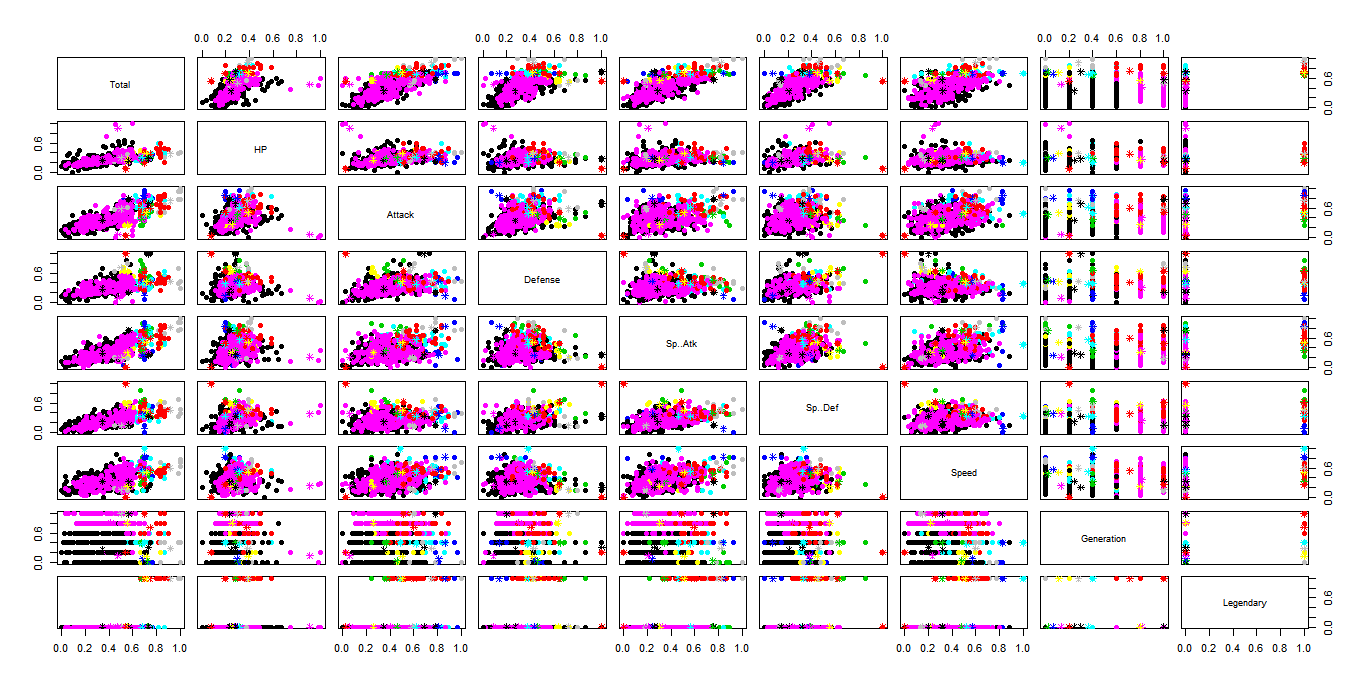
\includegraphics[width=1\columnwidth]{obrazki/graph_average} % Example image
	\end{center}
\end{figure}
\begin{figure}[H]
	\caption{Grupowanie metodą hierarchiczną średniego połączenia - dendrogram}
	\begin{center}
	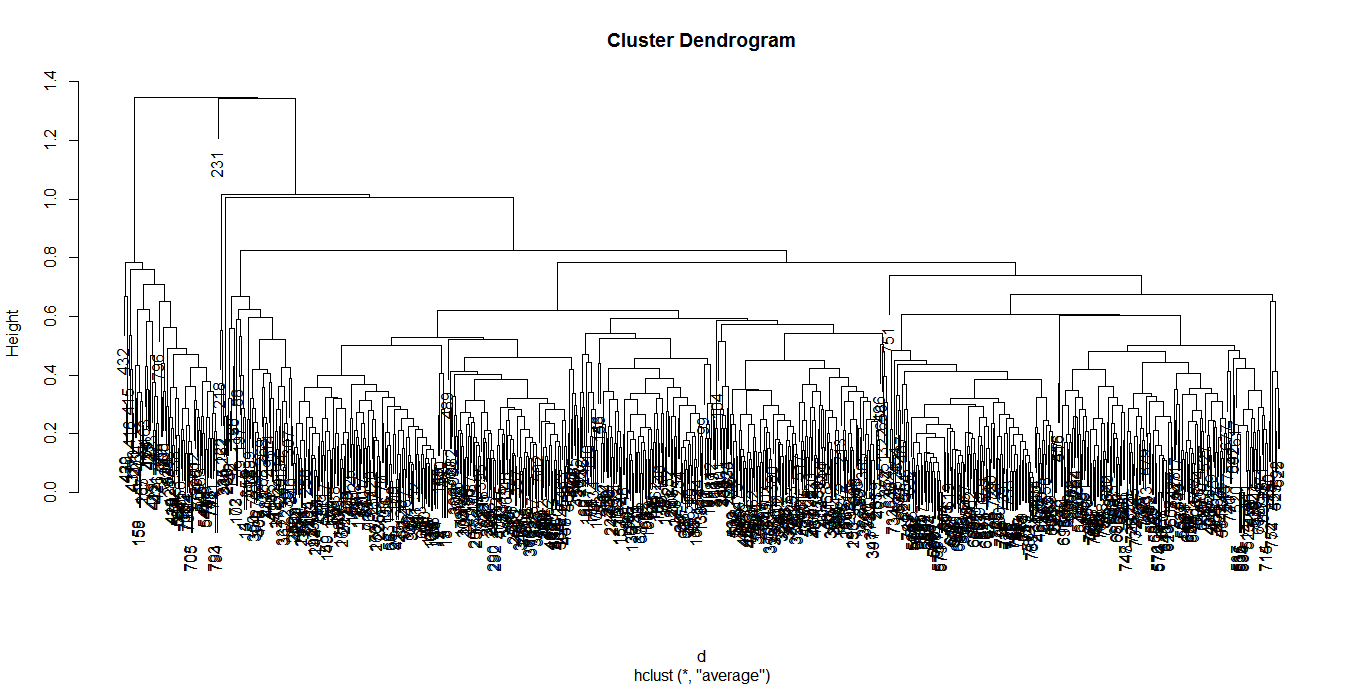
\includegraphics[width=1\columnwidth]{obrazki/dendrogram_average} % Example image
	\end{center}
\end{figure}
\begin{figure}[H]
	\caption{Grupowanie metodą hierarchiczną całkowitego połączenia}
	\begin{center}
	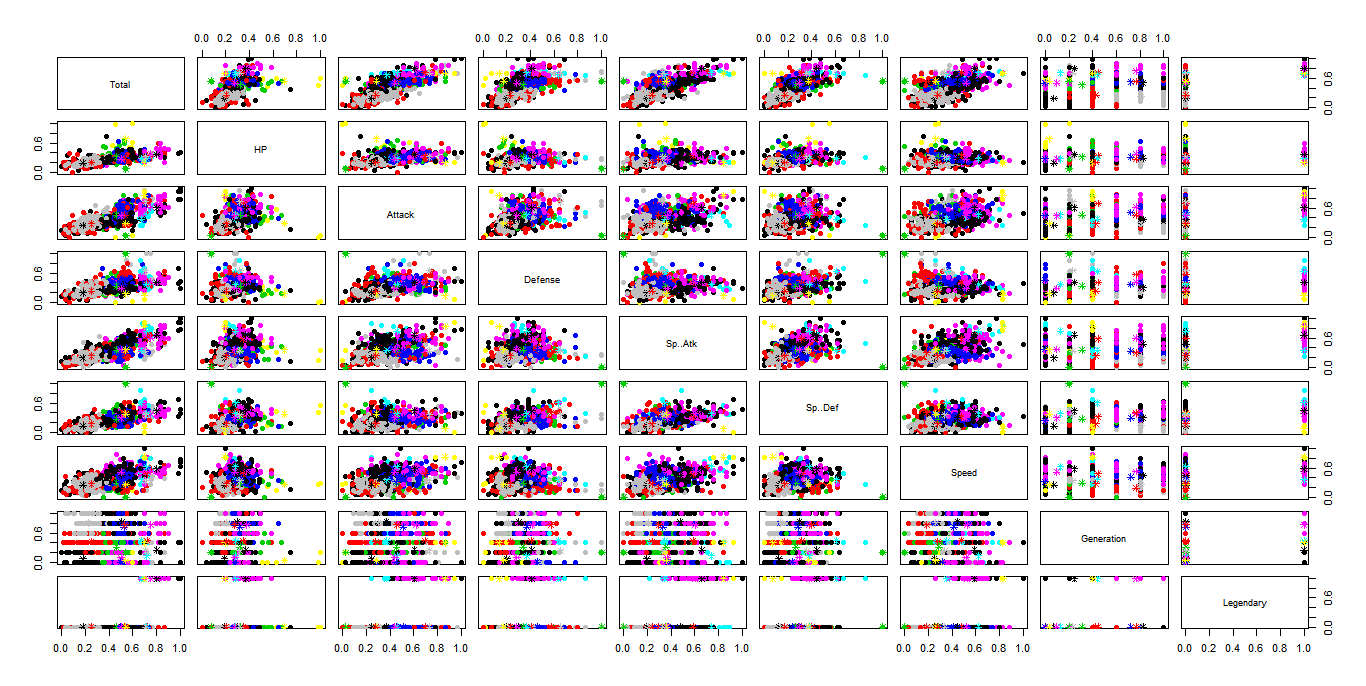
\includegraphics[width=1\columnwidth]{obrazki/graph_complete} % Example image
	\end{center}
\end{figure}
\begin{figure}[H]
	\caption{Grupowanie metodą hierarchiczną całkowitego połączenia - dendrogram}
	\begin{center}
	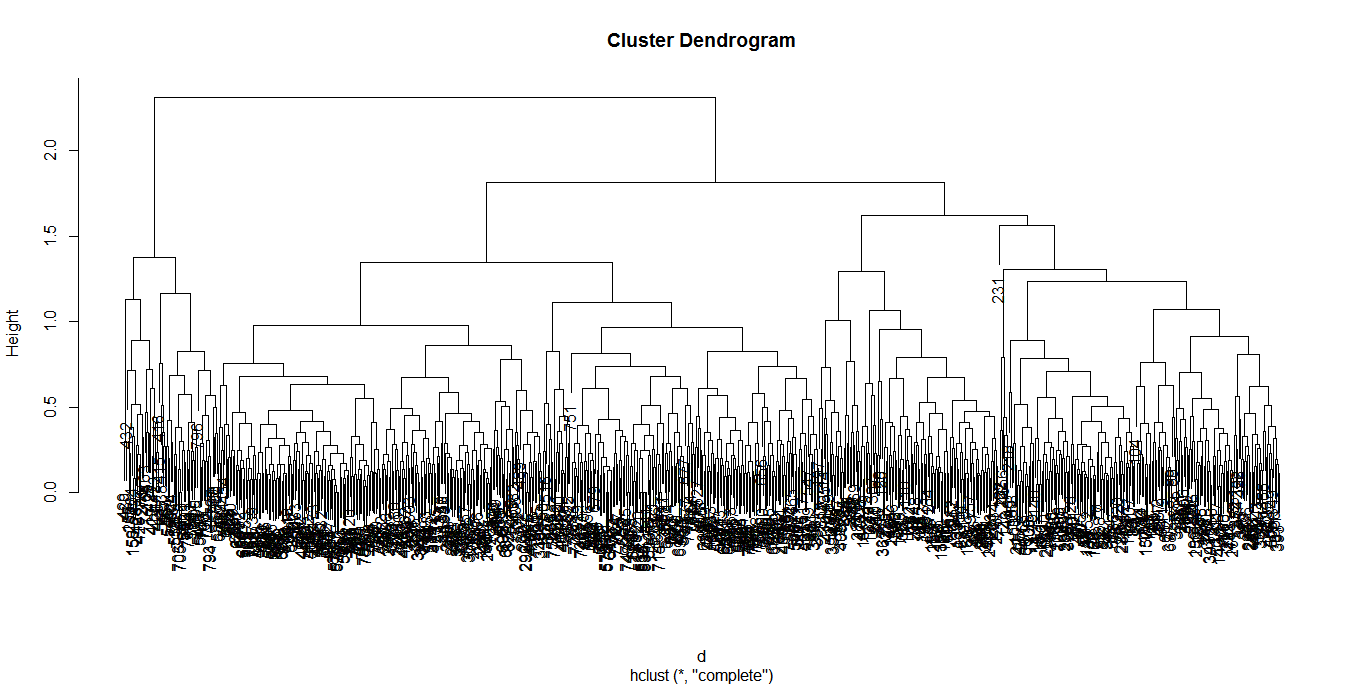
\includegraphics[width=1\columnwidth]{obrazki/dendrogram_complete} % Example image
	\end{center}
\end{figure}

Nasuwają się następujące wnioski.
\begin{itemize}
	\item Zróżnicowanie danych jest na tyle skomplikowane, że grupowanie nie wystarczy do poprawnego zaklasyfikowania danych. Jak widzieliśmy na Rysunku 1. dane nie są pogrupowane w tak równomierny sposób jaki sugerują powyższe wykresy.
	\item Ważną informację przekazują nam dendrogramy. Widzimy na nich, że jeśli bierzemy pod uwagę wszystkie parametry to wyodrębnić można jedną małą grupę i jedną dużą. Jest to odzwierciedlone na wykresach, gdzie widzimy zawsze jedno duże skupisko punktów oraz jedno mniejsze poboczne.
\end{itemize}
%----------------------------------------------------------------------------------------

\end{document}